\documentclass[main.tex]{subfiles}
\begin{document}
处理字的符的 Python 程序

\begin{figure}
	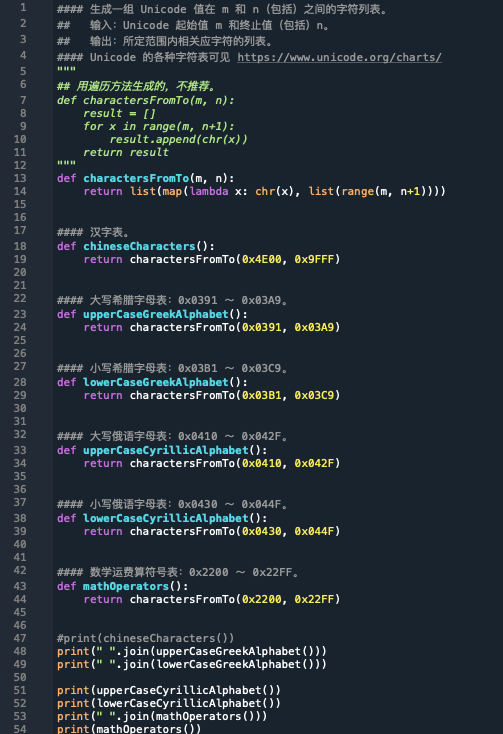
\includegraphics[viewport=0 0 490 735, clip]{string.png}
\end{figure}

Python 程序 xxx 生成希腊的字母如下:


从 Unicode 表中 Python 程序 xxx 生成部分常用数学运算速度符号如果下:


\begin{figure}
	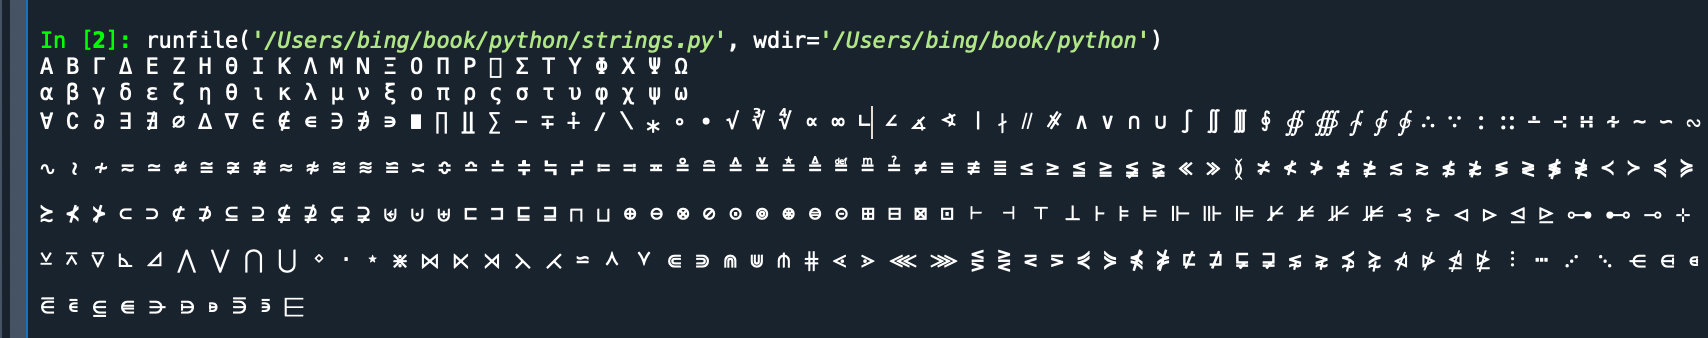
\includegraphics[viewport=0 0 490 200, clip]{greek_math_symbols.png}
\end{figure}

\begin{lstlisting}[language=Python]
import numpy as np
	
def incmatrix(genl1,genl2):
  m = len(genl1)
  n = len(genl2)
  M = None #to become the incidence matrix
  VT = np.zeros((n*m,1), int)  #dummy variable
	
  #compute the bitwise xor matrix
  M1 = bitxormatrix(genl1)
  M2 = np.triu(bitxormatrix(genl2),1) 

  for i in range(m-1):
for j in range(i+1, m):
  	[r,c] = np.where(M2 == M1[i,j])
	for k in range(len(r)):
	VT[(i)*n + r[k]] = 1;
	VT[(i)*n + c[k]] = 1;
	VT[(j)*n + r[k]] = 1;
	VT[(j)*n + c[k]] = 1;
	
	if M is None:
	M = np.copy(VT)
	else:
	M = np.concatenate((M, VT), 1)
	
	VT = np.zeros((n*m,1), int)
	
	return M
\end{lstlisting}

字符串处理

\newpage
\end{document} 